\documentclass{amsart}

\usepackage{tikz}
\usetikzlibrary{decorations.pathreplacing}
\usetikzlibrary{arrows}

\nofiles

\raggedbottom

%-------------------------------------------------------------------------------

\begin{document}

A point is defined as $\frac{1}{72}$ of an inch. Point size is defined as the number of points per em.

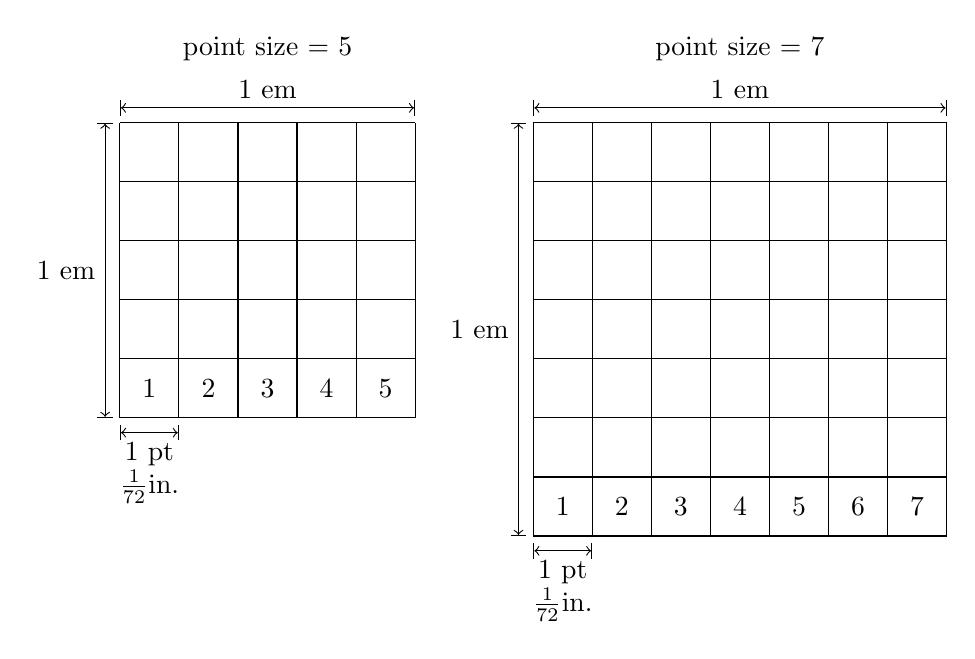
\begin{tikzpicture}[scale=.75]
\draw (2.5,6.25) node[anchor=center]{point size = 5};
\draw[step=1] (0,0) grid (5,5);

\draw (.5,.5) node[anchor=center]{1};
\draw (1.5,.5) node[anchor=center]{2};
\draw (2.5,.5) node[anchor=center]{3};
\draw (3.5,.5) node[anchor=center]{4};
\draw (4.5,.5) node[anchor=center]{5};

\draw[|<->|] (0,5.25) -- (5,5.25) node[above,midway] {1 em};
\draw[|<->|] (-.25,0) -- (-.25,5) node[left,midway] {1 em};
\draw[|<->|] (0,-.25) -- (1,-.25) node[below,text centered,text width=1cm,midway] {1 pt $\frac{1}{72}$in.};


\pgftransformxshift{7cm}
\pgftransformyshift{-2cm}
\draw (3.5,8.25) node[anchor=center]{point size = 7};
\draw[step=1] (0,0) grid (7,7);

\draw (.5,.5) node[anchor=center]{1};
\draw (1.5,.5) node[anchor=center]{2};
\draw (2.5,.5) node[anchor=center]{3};
\draw (3.5,.5) node[anchor=center]{4};
\draw (4.5,.5) node[anchor=center]{5};
\draw (5.5,.5) node[anchor=center]{6};
\draw (6.5,.5) node[anchor=center]{7};

\draw[|<->|] (0,7.25) -- (7,7.25) node[above,midway] {1 em};
\draw[|<->|] (-.25,0) -- (-.25,7) node[left,midway] {1 em};
\draw[|<->|] (0,-.25) -- (1,-.25) node[below,text centered,text width=1cm,midway] {1 pt $\frac{1}{72}$in.};
\end{tikzpicture}

UPM is the number of Font Units per em. It is also referred to as Em Size in Font Forge. The standard UPM for True Type is 2048. The standard UPM for PostScript is 1000.

\begin{align*}
\text{ppm} (\frac{\text{pixels}}{\text{em}})
&= \text{resolution} (\frac{\text{pixels}}{\text{inch}}) * \frac{1}{72} (\frac{\text{inch}}{\text{points}}) * \text{point size} (\frac{\text{points}}{\text{em}}) \\
\frac{\text{Font Units}}{\text{pixel}}
&= \text{UPM} (\frac{\text{Font Units}}{\text{em}}) * \frac{1}{\text{ppm}} (\frac{\text{em}}{\text{pixels}})
\end{align*}

\begin{center}
@2048 UPM, 96 dpi, 12 point size: 1 pixel = 128 Font Units
\end{center}

\end{document}

